\documentclass[11pt]{article}
\usepackage[letterpaper,margin=0.9in]{geometry}
\usepackage[T1]{fontenc}
\usepackage{lmodern,amsmath,amssymb,amsthm,mathtools,microtype,graphicx,tikz,enumitem,needspace}
\usepackage[colorlinks=true,linkcolor=black,urlcolor=blue!50!black]{hyperref}
\setlength{\parindent}{0pt}
\setlength{\parskip}{5pt plus 1pt minus 1pt}
\setlength{\emergencystretch}{2em}
\setlist{nosep,leftmargin=1.5em,topsep=4pt}
\newcommand{\Beta}{B}
\hypersetup{pdftitle={Illumination of orthogonal rooms with at most eight walls},pdfauthor={Daniel Wang and Peyton Wang}}
\title{Illumination of orthogonal rooms\\with at most eight walls}
\author{Daniel Wang \and Peyton Wang}
\date{Working draft v0.1 --- November 8, 2026}
\begin{document}
\maketitle
\begin{abstract}
Every finite strictly simple orthogonal polygon with at most eight maximal walls illuminates every pair of distinct interior points by a finite specular path avoiding every polygon corner. We present a constructive proof for arbitrary real dimensions and endpoints. A turning-angle classification gives six normal forms. Orientation-controlled paths in L rooms cover many endpoint placements; the remaining U, offset-corridor and staircase cases use explicit folding constructions. The staircase proof combines floor and roof charts whose sufficient inequalities exhaust all admissible metrics. Seam endpoints, rounding ties and potential floor or roof corner contacts are treated explicitly. There is no lattice or rationality assumption and no uniform bound on reflections is asserted. Historical priority is unconfirmed; no novelty claim is made.
\end{abstract}
\begin{center}\small Draft for external mathematical review. Not submitted or externally refereed.\end{center}
\section*{Reader's guide and provenance}
This manuscript typesets the corrected proof packet archived on November 8, 2026. Sections 0--8 retain that packet's numbering and proof text; display notation and typography are adapted for print. The proof is analytic. Fixed-input computations accompanying it are reproducibility controls and do not establish its real-parameter quantifiers.

Proof development and internal cross-review used Codex and Claude AI agents. A later coordinator review corrected a window-bound transcription and made seam cases, contact bounds and U-room termination explicit. No human mathematical referee or formal proof assistant has verified this work. Appendix A gives source links, reproduction instructions and the principal review checkpoints. Appendix B illustrates selected prescribed paths.

The result concerns at most \emph{eight walls}, equivalently at most two reflex corners. It does not address the separate eight-reflex-corner research target or the proposed universal 22-wall minimum. All point pairs in the theorem are interior pairs.
\section*{0. Conventions and statement}
\textbf{Room.} A room is a compact region \(P\) in the plane whose boundary is a Jordan polygon with every edge horizontal or vertical. "Strictly simple" means the boundary polygon has no self-contact. Suppress every vertex with a straight angle. The remaining vertices are the corners of \(P\), and the edges between consecutive corners are the maximal walls. \(W\) denotes the number of maximal walls, which equals the number of corners. A corner is convex if the interior angle is 90 degrees and reflex if it is 270 degrees.

\textbf{Interior point.} A point of the open set int(\(P\)). Points on an internal seam used in a proof are interior points of \(P\); points on a wall are not.

\textbf{Specular path.} Let \(S\) and \(T\) be distinct interior points. A specular path from \(S\) to \(T\) is a finite polygonal line \(S\) = \(p_{0}\), \(p_{1}\), ..., \(p_{n}\) = \(T\) such that:

\begin{enumerate}
\item Every open segment (\(p_{i}\), \(p_{i+1}\)) lies in int(\(P\)).
\item Every intermediate vertex \(p_{i}\), 0 < \(i\) < \(n\), lies in the relative interior of a maximal wall. In particular \(p_{i}\) is not a corner.
\item At every \(p_{i}\), 0 < \(i\) < \(n\), the direction obeys the reflection law: the velocity component normal to that wall reverses and the tangential component is unchanged.
\end{enumerate}
The path may pass through \(S\) or \(T\) at an intermediate time. If it passes through \(T\) at an intermediate time, truncating there gives a shorter path, so this convention loses nothing. Direct visibility, \(n\) = 1, counts as a path. "\(P\) illuminates (\(S\), \(T\))" means such a path exists.

\textbf{Folding maps.} For \(l\) > 0, \(F_{l}\) denotes the even, 2l-periodic triangular wave with \(F_{l}\)(\(z\)) = |\(z\)| for |\(z\)| \(\le\) \(l\). It satisfies \(F_{l}\)((2j+1)\(l\) + \(z\)) = \(l\) - |\(z\)| and \(F_{l}\)(2jl + \(z\)) = |\(z\)| for |\(z\)| \(\le\) \(l\) and integers \(j\). Unfolding a path that bounces between the walls \(x\) = 0 and \(x\) = \(l\) of a vertical strip is the same as applying \(F_{l}\) to a straight developed coordinate. Each crossing of a multiple of \(l\) is one reflection on a vertical wall, and the two velocity formulas agree on both sides of \(a\) fold, so condition 3 holds automatically at such a contact.

\Needspace{4\baselineskip}
\textbf{Main theorem.} Let \(P\) be a room with \(W\) \(\le\) 8. Then \(P\) illuminates every pair of distinct interior points.

The proof has seven parts. Section 1 classifies rooms with \(W\) \(\le\) 8 into six metric normal forms. Sections 2 to 6 prove illumination for each form. Section 7 assembles the theorem and lists the degeneracies that are covered explicitly.

\section*{1. Classification of rooms with at most eight walls}
\Needspace{4\baselineskip}
\textbf{Proposition 1.1.} Let \(P\) be a room with \(W\) maximal walls, \(c\) convex corners, and \(r\) reflex corners. Then \(c\) - \(r\) = 4 and \(c\) + \(r\) = \(W\), so \(W\) is even. For \(W\) \(\le\) 8 the only possibilities are \(W\) = 4 (rectangle), \(W\) = 6 (one reflex corner), and \(W\) = 8 (two reflex corners).

\emph{Proof.} Traverse the boundary counterclockwise. Each convex corner turns the tangent by +90 degrees and each reflex corner by -90 degrees. The total turning of a simple closed curve is 360 degrees, so \(c\) - \(r\) = 4. The two equations give \(r\) = (\(W\) - 4)/2, which is a nonnegative integer. The three cases follow.

\Needspace{4\baselineskip}
\textbf{Proposition 1.2 (normal forms).} After a Euclidean isometry, possibly including a reflection, every room with \(W\) \(\le\) 8 is one of the following, with all parameters arbitrary positive reals subject only to the displayed inequalities. Conversely every parameter choice satisfying the inequalities gives a room of the stated type.

\begin{itemize}
\item \textbf{Rectangle} (\(W\) = 4): [0, A] \(\times\) [0, \(C\)] with A, \(C\) > 0.
\item \textbf{\(L\)} (\(W\) = 6): \(P\) = ([0, A] \(\times\) [0, \(c\)]) union ([0, \(a\)] \(\times\) [\(c\), \(C\)]) with 0 < \(a\) < A and 0 < \(c\) < \(C\).
\item \textbf{\(U\)} (\(W\) = 8, reflex corners adjacent, \(k\) = 1): \(a\), \(b\), \(M\), \(c\) > 0, \(H_{L}\) > \(c\), \(H_{R}\) > \(c\), A = \(a\) + \(M\) + \(b\), with cyclic corners (0,0), (A,0), (A,\(H_{R}\)), (\(a\)+\(M\),\(H_{R}\)), (\(a\)+\(M\),\(c\)), (\(a\),\(c\)), (\(a\),\(H_{L}\)), (0,\(H_{L}\)).
\item \textbf{Staircase} (\(W\) = 8, \(k\) = 2): 0 < \(a\) < \(b\) < A and 0 < \(c\) < \(d\) < \(H\), \(P\) = ([0,A] \(\times\) [0,\(c\)]) union ([0,\(b\)] \(\times\) [\(c\),\(d\)]) union ([0,\(a\)] \(\times\) [\(d\),\(H\)]), corners (0,0), (A,0), (A,\(c\)), (\(b\),\(c\)), (\(b\),\(d\)), (\(a\),\(d\)), (\(a\),\(H\)), (0,\(H\)).
\item \textbf{\(T\) with independent floor heights} (\(W\) = 8, \(k\) = 3): 0 < \(a\) < \(b\) < A and 0 < \(u\), \(v\) < \(C\), \(P\) = ([0,\(a\)] \(\times\) [\(u\),\(C\)]) union ([\(a\),\(b\)] \(\times\) [0,\(C\)]) union ([\(b\),A] \(\times\) [\(v\),\(C\)]), corners (\(a\),0), (\(b\),0), (\(b\),\(v\)), (A,\(v\)), (A,\(C\)), (0,\(C\)), (0,\(u\)), (\(a\),\(u\)).
\item \textbf{Wide-middle offset corridor} (\(W\) = 8, \(k\) = 4): 0 < \(a\), \(B\) < A and 0 < \(b\) < \(c\) < \(C\), \(P\) = ([0,\(B\)] \(\times\) [0,\(b\)]) union ([0,A] \(\times\) [\(b\),\(c\)]) union ([\(a\),A] \(\times\) [\(c\),\(C\)]), corners (0,0), (\(B\),0), (\(B\),\(b\)), (A,\(b\)), (A,\(C\)), (\(a\),\(C\)), (\(a\),\(c\)), (0,\(c\)). The order of \(a\) and \(B\) is unrestricted. If \(a\) > \(B\) the two outer arms have disjoint horizontal projections.
\end{itemize}
Here \(k\) is the shorter cyclic distance, in edges, between the two reflex corners.

\emph{Proof.} \(W\) = 4 forces a rectangle. For \(W\) = 6 there is one reflex corner; the turn word is one minus sign and five plus signs, which fixes the six edge directions up to rotation and reflection. Positivity of the six edge lengths with two closure relations leaves four free parameters, and the displayed \(L\) realizes all of them.

For \(W\) = 8 there are two reflex corners among eight cyclic positions. Their shorter cyclic distance \(k\) is 1, 2, 3, or 4. A cyclic relabeling and, if needed, a reflection of the plane place the shorter arc first. Once \(k\) is fixed and the first edge direction is fixed, the six plus and two minus turns determine the entire edge-direction sequence. So each \(k\) has exactly one turn word up to these operations. For each word, the eight edge lengths satisfy two closure relations and leave six free parameters. The displayed vertex lists realize them:

\begin{itemize}
\item \(k\) = 1: directions \(R\), \(U\), \(L\), \(D\), \(L\), \(U\), \(L\), \(D\) with lengths A, \(H_{R}\), \(b\), \(H_{R}\) - \(c\), \(M\), \(H_{L}\) - \(c\), \(a\), \(H_{L}\). Positivity gives \(a\), \(b\), \(M\) > 0 and \(H_{L}\), \(H_{R}\) > \(c\). Horizontal closure is A = \(a\) + \(M\) + \(b\). Positivity of the displayed lengths alone does not imply \(c\) > 0. Strict simplicity supplies it: if \(c\) \(\le\) 0, the inner vertical wall \(x\) = \(a\) crosses or touches the non-adjacent bottom wall \(y\) = 0, since \(H_{L}\) > 0 and 0 < \(a\) < A. Thus \(c\) > 0.
\item \(k\) = 2: directions \(R\), \(U\), \(L\), \(U\), \(L\), \(U\), \(L\), \(D\) with lengths A, \(c\), A - \(b\), \(d\) - \(c\), \(b\) - \(a\), \(H\) - \(d\), \(a\), \(H\). Positivity gives exactly 0 < \(a\) < \(b\) < A and 0 < \(c\) < \(d\) < \(H\).
\item \(k\) = 3: directions \(R\), \(U\), \(R\), \(U\), \(L\), \(D\), \(R\), \(D\) with lengths \(b\) - \(a\), \(v\), A - \(b\), \(C\) - \(v\), A, \(C\) - \(u\), \(a\), \(u\). Positivity gives exactly 0 < \(a\) < \(b\) < A and 0 < \(u\), \(v\) < \(C\). No relation between \(u\) and \(v\) follows.
\item \(k\) = 4: directions \(R\), \(U\), \(R\), \(U\), \(L\), \(D\), \(L\), \(D\) with lengths \(B\), \(b\), A - \(B\), \(C\) - \(b\), A - \(a\), \(C\) - \(c\), \(a\), \(c\). Positivity gives exactly 0 < \(a\), \(B\) < A and 0 < \(b\), \(c\) < \(C\).
\end{itemize}
For \(k\) = 1, 2, 3 every positive parameter choice is strictly simple, because each displayed region is a union of axis-parallel rectangles glued along seams of positive length whose closure boundary is one Jordan curve. For \(k\) = 4 the non-adjacent edges \(x\) = \(B\) (0 \(\le\) \(y\) \(\le\) \(b\)) and \(y\) = \(c\) (0 \(\le\) \(x\) \(\le\) \(a\)) intersect if and only if \(B\) \(\le\) \(a\) and \(c\) \(\le\) \(b\). The opposite pair \(y\) = \(b\) (\(B\) \(\le\) \(x\) \(\le\) A) and \(x\) = \(a\) (\(c\) \(\le\) \(y\) \(\le\) \(C\)) intersects under the same condition. Every other non-adjacent pair has disjoint coordinate ranges. So the \(k\) = 4 polygon is strictly simple if and only if \(a\) < \(B\) or \(b\) < \(c\). If \(b\) \(\ge\) \(c\), then \(a\) < \(B\) holds, and the reflection across the line \(x\) = \(y\) gives new parameters A' = \(C\), \(B\)' = \(c\), \(a\)' = \(b\), \(b\)' = \(a\), \(c\)' = \(B\), \(C\)' = A with \(b\)' < \(c\)'. So the normal form with \(b\) < \(c\) covers every strictly simple \(k\) = 4 room. This proves the proposition.

The prescribed check \texttt{eight-wall-turn-check.py} enumerates the 28 labeled reflex-corner positions and verifies one representative polygon per class. That is a control on the combinatorics; the proof is the paragraph above.

\begin{figure}[htbp]\centering
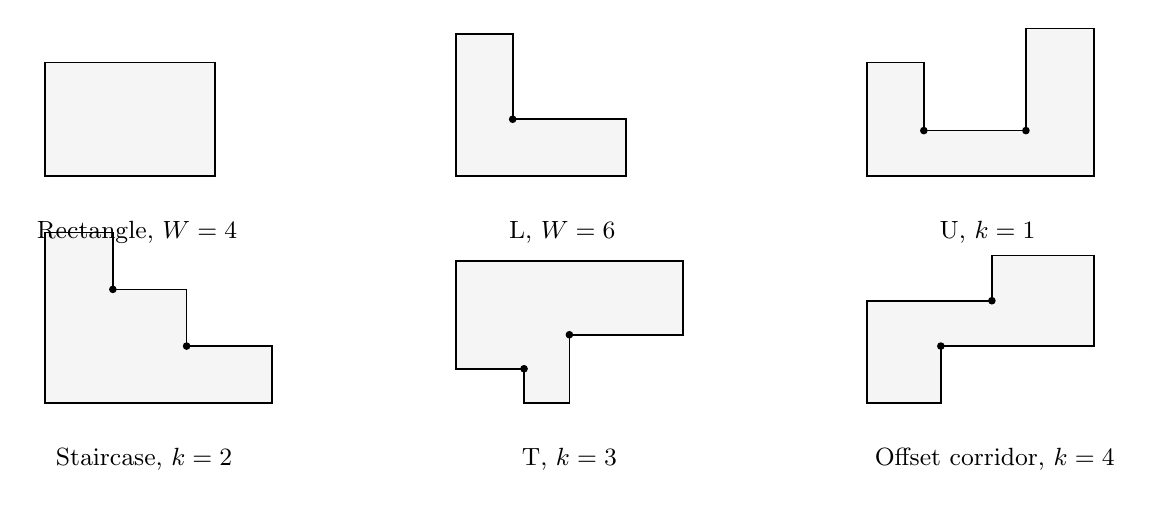
\begin{tikzpicture}[x=0.018cm,y=-0.018cm]
\filldraw[fill=gray!8,draw=black,line width=.6pt] (20.0,180.0) -- (140.0,180.0) -- (140.0,100.0) -- (20.0,100.0) -- cycle;
\filldraw[fill=gray!8,draw=black,line width=.6pt] (310.0,180.0) -- (430.0,180.0) -- (430.0,140.0) -- (350.0,140.0) -- (350.0,80.0) -- (310.0,80.0) -- cycle;
\filldraw[fill=gray!8,draw=black,line width=.6pt] (600.0,180.0) -- (760.0,180.0) -- (760.0,76.0) -- (712.0,76.0) -- (712.0,148.0) -- (640.0,148.0) -- (640.0,100.0) -- (600.0,100.0) -- cycle;
\filldraw[fill=gray!8,draw=black,line width=.6pt] (20.0,340.0) -- (180.0,340.0) -- (180.0,300.0) -- (120.0,300.0) -- (120.0,260.0) -- (68.0,260.0) -- (68.0,220.0) -- (20.0,220.0) -- cycle;
\filldraw[fill=gray!8,draw=black,line width=.6pt] (358.0,340.0) -- (390.0,340.0) -- (390.0,292.0) -- (470.0,292.0) -- (470.0,240.0) -- (310.0,240.0) -- (310.0,316.0) -- (358.0,316.0) -- cycle;
\filldraw[fill=gray!8,draw=black,line width=.6pt] (600.0,340.0) -- (652.0,340.0) -- (652.0,300.0) -- (760.0,300.0) -- (760.0,236.0) -- (688.0,236.0) -- (688.0,268.0) -- (600.0,268.0) -- cycle;
\fill (350.0,140.0) circle[radius=2.7];
\fill (712.0,148.0) circle[radius=2.7];
\fill (640.0,148.0) circle[radius=2.7];
\fill (120.0,300.0) circle[radius=2.7];
\fill (68.0,260.0) circle[radius=2.7];
\fill (390.0,292.0) circle[radius=2.7];
\fill (358.0,316.0) circle[radius=2.7];
\fill (652.0,300.0) circle[radius=2.7];
\fill (688.0,268.0) circle[radius=2.7];
\node[font=\small,anchor=north] at (85,205){Rectangle, $W=4$};
\node[font=\small,anchor=north] at (385,205){L, $W=6$};
\node[font=\small,anchor=north] at (685,205){U, $k=1$};
\node[font=\small,anchor=north] at (90,365){Staircase, $k=2$};
\node[font=\small,anchor=north] at (390,365){T, $k=3$};
\node[font=\small,anchor=north] at (690,365){Offset corridor, $k=4$};
\end{tikzpicture}
\caption{The six normal forms in Proposition 1.2. Black dots mark reflex corners. For eight-wall rooms, $k$ is the shorter cyclic edge distance between the two reflex corners. Drawings illustrate the classes; all dimensions in the theorem are arbitrary admissible positive reals.}
\end{figure}
\section*{2. Rectangles and \(L\) rooms}
Two interior points of a rectangle see each other directly. The \(L\) room needs the following theorem, which is used again in every eight-wall case.

\Needspace{4\baselineskip}
\textbf{Theorem 2.1 (\(L\), two orientations).} Let \(P\) = ([0,A] \(\times\) [0,\(c\)]) union ([0,\(a\)] \(\times\) [\(c\),\(C\)]) with 0 < \(a\) < A and 0 < \(c\) < \(C\), and let \(s\), \(t\) be distinct interior points. There is a specular path from \(s\) to \(t\) that reflects only on vertical walls and whose \(y\) coordinate is monotone. There is also one that reflects only on horizontal walls and whose \(x\) coordinate is monotone. A direct segment counts as both.

\emph{Proof.} \(P\) is the union of the convex rectangles \(R_{1}\) = [0,A] \(\times\) [0,\(c\)] and \(R_{2}\) = [0,\(a\)] \(\times\) [0,\(C\)]. If \(s\) and \(t\) lie in a common \(R_{i}\), the segment between them lies in that rectangle. Interior points of \(P\) on the seam \(y\) = \(c\) (0 < \(x\) < \(a\)) or on the line \(x\) = \(a\) (0 < \(y\) < \(c\)) belong to both rectangles, so the segment lies in int(\(P\)) except for its endpoints. This covers every placement except, after relabeling,

\begin{gather*}
s = (x_{s}, y_{s}) \text{with}\; a < x_{s} < A, 0 < y_{s} < c \\
t = (x_{t}, y_{t}) \text{with}\; 0 < x_{t} < a, c < y_{t} < C
\end{gather*}
Write \(D_{s}\) = \(c\) - \(y_{s}\) > 0, \(D_{t}\) = \(y_{t}\) - \(c\) > 0, \(r\) = \(D_{t}\) / \(D_{s}\). The images of \(x_{t}\) under the reflections of the upper strip [0,\(a\)] form

\begin{gather*}
E = \{ e x_{t} + 2ma : e \in \{+1,-1\}, m \in \mathbb{Z} \}
\end{gather*}
\(E\) is symmetric under negation. Its consecutive gaps alternate between 2x\_t and 2(\(a\) - \(x_{t}\)); both are strictly less than 2a.

Put \(h\) = -\(r\) \(x_{s}\) and choose \(x\) in \(E\) with 0 < |\(x\) - \(h\)| \(\le\) \(a\). Such \(x\) exists: if \(h\) is not in \(E\), the nearest point of \(E\) is at distance less than \(a\); if \(h\) is in \(E\), its nearer neighbor is at distance 2 min(\(x_{t}\), \(a\) - \(x_{t}\)) \(\le\) \(a\).

If \(x\) > \(h\) set \(X_{s}\) = \(x_{s}\), \(X_{t}\) = \(x\); if \(x\) < \(h\) set \(X_{s}\) = -\(x_{s}\), \(X_{t}\) = -\(x\). In both cases \(X_{t}\) is in \(E\). The straight developed segment from (\(X_{s}\), \(y_{s}\)) to (\(X_{t}\), \(y_{t}\)) crosses \(y\) = \(c\) at

\begin{gather*}
q = (r X_{s} + X_{t})/(1 + r) = |x - h|/(1 + r)
\end{gather*}
so 0 < \(q\) \(\le\) \(a\)/(1+\(r\)) < \(a\). The crossing is strictly inside the open seam.

Fold the segment into \(P\). Below \(y\) = \(c\) the developed \(x\) runs from \(X_{s}\) to \(q\) and stays in (-A, A). If \(X_{s}\) = \(x_{s}\) there is no reflection. If \(X_{s}\) = -\(x_{s}\) the segment crosses \(x\) = 0 exactly once, at a height strictly between \(y_{s}\) and \(c\); reflecting the negative part in \(x\) = 0 gives one smooth contact on the wall \(x\) = 0. Above \(y\) = \(c\) apply \(F_{a}\). The portal value \(q\) is fixed because 0 < \(q\) < \(a\), and the final value is \(F_{a}\)(\(X_{t}\)) = \(x_{t}\). Each crossing of a multiple of \(a\) is one reflection on \(x\) = 0 or \(x\) = \(a\), at a height strictly between \(c\) and \(y_{t}\) < \(C\), so never at a corner. The developed segment is finite, so there are finitely many folds. The \(y\) coordinate increases strictly, so no horizontal wall is touched, and the seam crossing at (\(q\), \(c\)) is an interior point. This is the vertical-only path.

Exchanging the coordinates maps \(P\) to an \(L\) of the same form with parameters (A', \(a\)', \(c\)', \(C\)') = (\(C\), \(c\), \(a\), A). The construction gives a path from \(t\) to \(s\) whose original \(x\) coordinate is monotone and which reflects only on horizontal walls. Reverse it.

\Needspace{4\baselineskip}
\textbf{Lemma 2.2 (source on the base).} In the \(L\) of Theorem 2.1 let the source be (\(x\), 0) with 0 < \(x\) < A on the base and the target (\(t\), \(y\)) with 0 < \(t\) < \(a\) and \(c\) < \(y\) < \(C\). Then there is a vertical-only specular path from (\(x\), 0) to (\(t\), \(y\)) whose \(y\) coordinate increases strictly, with no contact on the base after the starting point.

\emph{Proof.} If \(x\) \(\le\) \(a\), the segment lies in the column [0,\(a\)] \(\times\) [0,\(C\)]; after its start its \(x\) coordinate is strictly less than \(a\) when \(x\) = \(a\), because \(t\) < \(a\). If \(a\) < \(x\) < A, repeat the proof of Theorem 2.1 with \(y_{s}\) = 0: \(r\) = (\(y\) - \(c\))/\(c\), \(h\) = -\(r\) \(x\), choose \(x\)' in \(E\) with 0 < |\(x\)' - \(h\)| \(\le\) \(a\), and \(q\) = |\(x\)' - \(h\)|/(1+\(r\)) in (0, \(a\)). The lower fold crosses \(x\) = 0 at most once, at a height strictly between 0 and \(c\). Everything else is unchanged. The source height was used in Theorem 2.1 only to make the source interior, not in any inequality.

Lemma 2.2 is used where \(a\) base of an \(L\) subroom is an internal seam of a larger room, so that (\(x\), 0) is an interior point of that room. It never admits a boundary point of the actual room as an endpoint.

\Needspace{4\baselineskip}
\textbf{Corollary 2.3.} Every \(L\) room illuminates every pair of distinct interior points.

\section*{3. \(U\) rooms (\(k\) = 1)}
Fix \(a\), \(b\), \(M\), \(c\) > 0, \(H_{L}\), \(H_{R}\) > \(c\), A = \(a\) + \(M\) + \(b\), and the \(U\) room of Proposition 1.2. The left arm is [0,\(a\)] \(\times\) [0,\(H_{L}\)], the right arm is [\(a\)+\(M\), A] \(\times\) [0,\(H_{R}\)], and the bottom rectangle is [0,A] \(\times\) [0,\(c\)]. Interior points on the level \(y\) = \(c\) have 0 < \(x\) < \(a\) or \(a\) + \(M\) < \(x\) < A.

\Needspace{4\baselineskip}
\textbf{Theorem 3.1 (opposite arms).} Let \(s\) = (\(x_{s}\), \(y_{s}\)) with 0 < \(x_{s}\) < \(a\) and \(c\) \(\le\) \(y_{s}\) < \(H_{L}\), and \(t\) = (\(a\) + \(M\) + \(x_{t}\), \(y_{t}\)) with 0 < \(x_{t}\) < \(b\) and \(c\) \(\le\) \(y_{t}\) < \(H_{R}\). There is a specular path from \(s\) to \(t\) that reflects exactly once on the floor \(y\) = 0, at a point with \(x\) in (\(M\)/2, A - \(M\)/2), and otherwise only on vertical walls.

\emph{Proof.} Step 1, arm lengths. For \(\tau\) > 0 define

\begin{gather*}
L_{n} = a - x_{s} + 2na,   R_{m} = x_{t} + 2mb,   n, m \ge  0 \\
L(\tau) = \text{the}\; \text{first}\; L_{n} \text{strictly}\; \text{greater}\; \text{than}\; (y_{s} - c) \tau \\
R(\tau) = \text{the}\; \text{first}\; R_{m} \text{strictly}\; \text{greater}\; \text{than}\; (y_{t} - c) \tau
\end{gather*}
Both are nondecreasing, right-continuous step functions of \(\tau\). Put

\begin{gather*}
l_{s} = L(\tau) - (y_{s} - c) \tau \in (0, 2a] \\
l_{t} = R(\tau) - (y_{t} - c) \tau \in (0, 2b]
\end{gather*}
A remainder equals its upper bound exactly at a jump of its step function. If \(y_{s}\) = \(c\) then \(L\) is the constant \(L_{0}\) = \(a\) - \(x_{s}\) and \(l_{s}\) = \(a\) - \(x_{s}\); likewise for \(y_{t}\) = \(c\).

Step 2, a fixed point. Choose \(\tau_{0}\) > 2 max(\(a\), \(b\))/\(c\) and an integer \(k\) \(\ge\) 0 with \(B\) = \(M\) + 2kA > 2c \(\tau_{0}\). Put \(\Sigma\) = \(y_{s}\) + \(y_{t}\) and

\begin{gather*}
H(\tau) = (L(\tau) + R(\tau) + B)/\Sigma
\end{gather*}
Then \(\Sigma\) \(\tau\) - \(L\)(\(\tau\)) - \(R\)(\(\tau\)) = 2c \(\tau\) - \(l_{s}\) - \(l_{t}\), so \(H\)(\(\tau\)) > \(\tau\) if and only if \(B\) + \(l_{s}\) + \(l_{t}\) > 2c \(\tau\). This holds at \(\tau_{0}\). \(H\) is nondecreasing, so the iterates \(\tau_{j+1}\) = \(H\)(\(\tau_{j}\)) are nondecreasing. They are bounded by \(\tau_{\mathrm{max}}\) = (\(B\) + 2a + 2b)/(2c), because 2c \(\tau_{\mathrm{max}}\) \(\ge\) \(B\) + \(l_{s}\) + \(l_{t}\) gives \(H\)(\(\tau_{\mathrm{max}}\)) \(\le\) \(\tau_{\mathrm{max}}\). On [\(\tau_{0}\), \(\tau_{\mathrm{max}}\)] only finitely many values of (\(L\), \(R\)) occur, so the iteration is stationary after finitely many steps. Let \(\tau_{n}\) be the first stationary iterate; \(n\) \(\ge\) 1 and \(\tau_{n}\) > \(\tau_{n-1}\).

The fixed point is not a jump of \(L\). If it were, then \(L\)(\(\tau_{n-1}\)) \(\le\) \(L\)(\(\tau_{n}\)) - 2a and \(R\)(\(\tau_{n-1}\)) \(\le\) \(R\)(\(\tau_{n}\)), so \(H\)(\(\tau_{n-1}\)) < \(H\)(\(\tau_{n}\)) = \(\tau_{n}\), contradicting \(\tau_{n}\) = \(H\)(\(\tau_{n-1}\)). The same argument applies to \(R\). Hence at \(\tau\) = \(\tau_{n}\) one has 0 < \(l_{s}\) < 2a and 0 < \(l_{t}\) < 2b, together with the fixed-point relation \(\Sigma\) \(\tau\) = \(L\) + \(R\) + \(B\), which is equivalent to

\begin{gather*}
2c \tau = B + l_{s} + l_{t}.                                   (3.1)
\end{gather*}
The iteration also has an explicit finite bound. Write \(f_{s}\) = \(y_{s}\) - \(c\) and \(f_{t}\) = \(y_{t}\) - \(c\), and let \(n_{L}\)(\(\tau\)), \(n_{R}\)(\(\tau\)) be the selected indices in Step 1. They are nonnegative and nondecreasing. For \(j\) \(\ge\) 1, if \(\tau_{j+1}\) > \(\tau_{j}\), the identity \(\tau_{j}\) = \(H\)(\(\tau_{j-1}\)) implies \(H\)(\(\tau_{j}\)) > \(H\)(\(\tau_{j-1}\)); hence at least one selected index increases. Consequently the first fixed point is reached in at most

\begin{gather*}
1 + n_{L}(\tau_{\mathrm{max}}) + n_{R}(\tau_{\mathrm{max}}) \\
\le  3 + \operatorname{floor}(f_{s} \tau_{\mathrm{max}}/(2a)) + \operatorname{floor}(f_{t} \tau_{\mathrm{max}}/(2b))
\end{gather*}
updates from \(\tau_{0}\). The first bound may overcount indices already present at \(\tau_{0}\). The inequalities follow directly from the first-strictly-greater selection rule and 0 < \(a\) - \(x_{s}\) < \(a\), 0 < \(x_{t}\) < \(b\). No convergence or continuity at a step-function jump is assumed.

Step 3, portals. Define the portal heights

\begin{gather*}
u = y_{s} - L/\tau = c - l_{s}/\tau,   v = y_{t} - R/\tau = c - l_{t}/\tau
\end{gather*}
Since \(\tau\) > \(\tau_{0}\) > 2 max(\(a\),\(b\))/\(c\), both lie in (0, \(c\)). From (3.1), \(u\) + \(v\) = \(B\)/\(\tau\).

Step 4, the left arm. From \(s\) travel with velocity (1, -1/\(\tau\)) in the developed left strip and fold with \(F_{a}\). The developed horizontal distance to the exit is \(L\) = \(a\) - \(x_{s}\) + 2n'\(a\) for some \(n\)' \(\ge\) 0, so the path reaches \(x\) = \(a\) moving right after \(n\)' full round trips, at height \(u\). Every earlier contact with \(x\) = \(a\) is at least 2a developed units before the exit, at height at least \(u\) + 2a/\(\tau\) = \(c\) + (2a - \(l_{s}\))/\(\tau\) > \(c\). Every contact with \(x\) = 0 is at a height strictly between \(u\) and \(y_{s}\). All contacts with \(x\) = 0 lie at heights strictly between \(u\) > 0 and \(y_{s}\) < \(H_{L}\). All earlier contacts with \(x\) = \(a\) lie strictly above \(c\) and below \(y_{s}\) < \(H_{L}\). Thus every contact is on \(a\) genuine smooth wall, none is a corner, and the roof is never touched. When \(y_{s}\) = \(c\), the path goes directly from \(s\) to (\(a\), \(u\)) with no contact. The path leaves the left arm through the open passage \{\(a\)\} \(x\) (0, \(c\)) at (\(a\), \(u\)), moving right and down.

Step 5, the bottom strip. For developed distance 0 \(\le\) \(d\) \(\le\) \(B\) from (\(a\), \(u\)), set \(X\)(\(d\)) = \(a\) + \(d\), \(Y\)(\(d\)) = \(u\) - \(d\)/\(\tau\), and take the physical point (\(F_{A}\)(\(X\)(\(d\))), |\(Y\)(\(d\))|). Since \(a\) + \(B\) = \(a\) + \(M\) + 2kA and 2kA is an even multiple of A, \(F_{A}\)(\(a\) + \(B\)) = \(a\) + \(M\), and after 2k vertical folds the horizontal velocity is again positive. The developed height at \(d\) = \(B\) is \(u\) - \(B\)/\(\tau\) = -\(v\), so the physical endpoint is (\(a\) + \(M\), \(v\)) moving right and up. \(Y\) vanishes exactly once, at \(d_{0}\) = \(u\) \(\tau\), where the developed coordinate is

\begin{gather*}
X_{0} = a + u \tau = a + c \tau - l_{s} = a + (B + l_{s} + l_{t})/2 - l_{s} \\
= a + M/2 + kA + (l_{t} - l_{s})/2
\end{gather*}
Since -\(a\) < (\(l_{t}\) - \(l_{s}\))/2 < \(b\), \(X_{0}\) lies strictly between kA + \(M\)/2 and kA + A - \(M\)/2, so \(X_{0}\) is not a multiple of A and the physical floor contact \(F_{A}\)(\(X_{0}\)) lies in (\(M\)/2, A - \(M\)/2). It is a smooth point of the floor, at which the vertical velocity reverses and the horizontal velocity is unchanged. Every vertical-wall contact in the strip is at developed \(X\) in A \(\mathbb{Z}\), hence at nonzero height |\(Y\)| \(\le\) max(\(u\), \(v\)) < \(c\), on the walls \(x\) = 0 or \(x\) = A below the level \(c\). So the strip path stays in the bottom rectangle below \(y\) = \(c\), avoids the notch wall \(y\) = \(c\) and both inner walls, and touches no corner.

Step 6, the right arm. The mirror image of Step 4 carries the path from (\(a\) + \(M\), \(v\)), moving right and up, through developed distance \(R\) = \(x_{t}\) + 2mb to \(t\). Earlier contacts with \(x\) = \(a\) + \(M\) are at heights above \(c\), and contacts with \(x\) = A are at heights strictly between \(v\) and \(y_{t}\) < \(H_{R}\).

At both portals the arm formula and the strip formula are the same affine function folded by compatible maps, so positions and velocities match. All contacts are ordinary reflections, there are finitely many of them, and the path ends at \(t\). Its number of reflections is exactly

\begin{gather*}
2 n_{L}(\tau) + 2 n_{R}(\tau) + 2k + 1
\end{gather*}
counting the two arm strips, the 2k bottom-strip vertical contacts, and the single floor contact. In particular it is at most

\begin{gather*}
2 \operatorname{floor}(f_{s} \tau_{\mathrm{max}}/(2a)) + 2 \operatorname{floor}(f_{t} \tau_{\mathrm{max}}/(2b)) + 2k + 5
\end{gather*}
One may fix \(\tau_{0}\) and \(k\) from the room dimensions alone, then replace \(f_{s}\) and \(f_{t}\) in this upper bound by \(H_{L}\) - \(c\) and \(H_{R}\) - \(c\). This gives a finite room-dependent bound for all opposite-arm endpoint pairs. No bound uniform over all room metrics is asserted.

\Needspace{4\baselineskip}
\textbf{Theorem 3.2.} Every \(U\) room illuminates every pair of distinct interior points.

\emph{Proof.} Classify the two points. If both lie in one arm column [0,\(a\)] \(x\) (0,\(H_{L}\)) or (\(a\)+\(M\), A) \(x\) (0,\(H_{R}\)), they see each other. If at least one point has \(y\) < \(c\) and both have \(y\) \(\le\) \(c\), both lie in the bottom rectangle and the segment between them is interior, because a point with \(y\) = \(c\) is interior only over an open mouth. If both have \(y\) \(\ge\) \(c\) and lie in different arms, Theorem 3.1 applies, including one or both heights equal to \(c\). The remaining case is one point with \(y\) > \(c\) in one arm, say the left, and the other with \(y\) < \(c\). Then both are interior points of the \(L\) subroom \(Q\) = ([0,A] \(\times\) [0,\(c\)]) union ([0,\(a\)] \(\times\) [\(c\),\(H_{L}\)]). Every vertical wall of \(Q\) is a wall of \(P\). The only part of the boundary of \(Q\) that is not on the boundary of \(P\) is the segment \(y\) = \(c\), \(a\) + \(M\) < \(x\) < A, which contains the reflex corner (\(a\) + \(M\), \(c\)) of \(P\) as a smooth point. The vertical-only path of Theorem 2.1 touches no horizontal wall of \(Q\), so it is a specular path in \(P\). The case of the right arm is symmetric.

\section*{4. \(T\) rooms with independent floor heights (\(k\) = 3)}
Fix 0 < \(a\) < \(b\) < A, 0 < \(u\), \(v\) < \(C\), and \(P\) = ([0,\(a\)] \(\times\) [\(u\),\(C\)]) union ([\(a\),\(b\)] \(\times\) [0,\(C\)]) union ([\(b\),A] \(\times\) [\(v\),\(C\)]).

\Needspace{4\baselineskip}
\textbf{Theorem 4.1.} \(P\) illuminates every pair of distinct interior points.

\emph{Proof.} Assign each interior point to the left wing (\(x\) \(\le\) \(a\)), the stem (\(a\) < \(x\) < \(b\)), or the right wing (\(x\) \(\ge\) \(b\)). An interior point with \(x\) = \(a\) has \(y\) > \(u\) and one with \(x\) = \(b\) has \(y\) > \(v\).

Two points in one class see each other, because each class lies in a convex rectangle contained in \(P\): [0,\(a\)] \(\times\) [\(u\),\(C\)], [\(a\),\(b\)] \(\times\) [0,\(C\)], or [\(b\),A] \(\times\) [\(v\),\(C\)]. A segment along \(x\) = \(a\) or \(x\) = \(b\) has both endpoint heights above the corresponding floor and is interior.

Stem and left wing. Use the \(L\) subroom

\begin{gather*}
Q_{L} = ([0,b] \times [u,C]) \cup ([a,b] \times [0,u])
\end{gather*}
After the isometry (\(x\), \(y\)) \(\to\) (\(b\) - \(x\), \(C\) - \(y\)) it has the form of Theorem 2.1. Both points are interior to \(Q_{L}\), including a left-wing point on \(x\) = \(a\). Take the horizontal-only path. The horizontal walls of \(Q_{L}\), namely \(y\) = \(C\) over [0,\(b\)], \(y\) = \(u\) over [0,\(a\)], and \(y\) = 0 over [\(a\),\(b\)], are walls of \(P\). The vertical boundary \(x\) = \(b\) of \(Q_{L}\) is partly artificial (\(v\) < \(y\) < \(C\)) and contains the reflex corner (\(b\), \(v\)) of \(P\) as a smooth point; the chosen path never touches a vertical wall. So it is a specular path in \(P\). Stem and right wing use \(Q_{R}\) = ([\(a\),A] \(\times\) [\(v\),\(C\)]) union ([\(a\),\(b\)] \(\times\) [0,\(v\)]) in the same way.

Opposite wings. Reflect across a vertical line if needed so that \(u\) \(\le\) \(v\). Let \(S\) = (\(x_{s}\), \(y_{s}\)) with 0 < \(x_{s}\) \(\le\) \(a\), \(u\) < \(y_{s}\) < \(C\), and \(T\) = (\(x_{t}\), \(y_{t}\)) with \(b\) \(\le\) \(x_{t}\) < A, \(v\) < \(y_{t}\) < \(C\). If \(y_{s}\) \(\ge\) \(v\) the segment lies in the rectangle [0,A] \(\times\) [\(v\),\(C\)]; its open part has \(y\) > \(v\) because \(y_{t}\) > \(v\). Otherwise \(u\) < \(y_{s}\) < \(v\). Use the \(L\) subroom

\begin{gather*}
Q = ([0,A] \times [v,C]) \cup ([0,b] \times [u,v])
\end{gather*}
which after \(y\) \(\to\) \(C\) - \(y\) has the form of Theorem 2.1. Both points are interior to \(Q\). Its vertical walls \(x\) = 0 (\(u\) \(\le\) \(y\) \(\le\) \(C\)), \(x\) = A (\(v\) \(\le\) \(y\) \(\le\) \(C\)), and \(x\) = \(b\) (\(u\) \(\le\) \(y\) \(\le\) \(v\)) are walls of \(P\). Its only artificial boundary is \(y\) = \(u\) over (\(a\), \(b\)), which contains the reflex corner (\(a\), \(u\)) as a smooth point. The vertical-only path of Theorem 2.1 touches no horizontal wall, so it is a specular path in \(P\). The case \(u\) > \(v\) is the mirror image.

These cases exhaust all placements, including every seam and floor-level equality.

The equal-floor \(T\) room (\(u\) = \(v\)) is a special case of Theorem 4.1.

\section*{5. Wide-middle offset corridors (\(k\) = 4)}
Fix 0 < \(a\), \(B\) < A, 0 < \(b\) < \(c\) < \(C\), and \(P\) = ([0,\(B\)] \(\times\) [0,\(b\)]) union ([0,A] \(\times\) [\(b\),\(c\)]) union ([\(a\),A] \(\times\) [\(c\),\(C\)]). Write \(W\) = A - \(a\) and \(g\) = \(c\) - \(b\). Interior points on the seam \(y\) = \(b\) have 0 < \(x\) < \(B\); interior points on the seam \(y\) = \(c\) have \(a\) < \(x\) < A.

\Needspace{4\baselineskip}
\textbf{Theorem 5.1 (opposite arms).} Let \(S\) = (\(x_{s}\), \(y_{s}\)) with 0 < \(x_{s}\) < \(B\), 0 < \(y_{s}\) < \(b\), and \(T\) = (\(x_{t}\), \(y_{t}\)) with \(a\) < \(x_{t}\) < A, \(c\) < \(y_{t}\) < \(C\). There is a specular path from \(S\) to \(T\) with strictly increasing \(y\) coordinate that reflects only on vertical walls.

\emph{Proof.} Step 1, reduction to \(B\) \(\ge\) \(W\). Rotating \(P\) by 180 degrees about its center gives a room of the same form with the roles of \(B\) and \(W\) exchanged and \(g\) unchanged. The rotation exchanges \(S\) and \(T\) and preserves specular paths. So assume \(B\) \(\ge\) \(W\).

Step 2, windows. Put \(H_{s}\) = \(b\) - \(y_{s}\), \(H_{t}\) = \(y_{t}\) - \(c\), \(D\) = \(H_{s}\) + \(g\) + \(H_{t}\). Choose an integer \(k\) \(\ge\) 0 so large that, with \(K\) = (2k+1)A,

\begin{gather*}
(H_{s} K + g x_{s})/(2Bg) \ge  1
\end{gather*}
and let \(n\) be a nearest integer to this quantity; then \(n\) \(\ge\) 1 and

\begin{gather*}
|g \theta - K| \le  Bg/H_{s},   \text{where}\; \theta = (2nB - x_{s})/H_{s}.            (5.1)
\end{gather*}
The slopes \(\tau\) for which the developed point \(z\) = \(x_{s}\) + \(H_{s}\) \(\tau\) - 2nB lies in (-\(B\), \(B\)) form the open interval I = ((2nB - \(x_{s}\) - \(B\))/\(H_{s}\), (2nB - \(x_{s}\) + \(B\))/\(H_{s}\)), which is entirely positive since \(n\) \(\ge\) 1 and \(x_{s}\) < \(B\). The affine map \(U\)(\(\tau\)) = \(x_{s}\) + (\(H_{s}\) + \(g\)) \(\tau\) - 2nB sends I onto (\(g\) \(\theta\) - \(R\), \(g\) \(\theta\) + \(R\)) with \(R\) = \(B\)(\(H_{s}\) + \(g\))/\(H_{s}\). By (5.1) and \(B\) \(\ge\) \(W\),

\begin{gather*}
|K - g \theta| + W \le  Bg/H_{s} + W \le  R
\end{gather*}
so the open window (\(K\) - \(W\), \(K\) + \(W\)) lies inside \(U\)(I). Its preimage

\begin{gather*}
J = ((2nB + K - x_{s} - W)/(H_{s} + g), (2nB + K - x_{s} + W)/(H_{s} + g))
\end{gather*}
is a nonempty open subinterval of I. For every \(\tau\) in \(J\),

\begin{gather*}
|z| < B,   z = x_{s} + H_{s} \tau - 2nB,                               (5.2) \\
|w| < W,   w = x_{s} + (H_{s} + g) \tau - 2nB - K.                     (5.3)
\end{gather*}
Step 3, the target image. Put \(Y\) = A - \(x_{t}\), so 0 < \(Y\) < \(W\). On \(J\) the affine coordinate \(Z\)(\(\tau\)) = \(x_{s}\) + \(D\) \(\tau\) - 2nB - \(K\) = \(w\) + \(H_{t}\) \(\tau\) runs over an open interval (\(Z_{\mathrm{lo}}\), \(Z_{\mathrm{hi}}\)) of length 2W \(D\)/(\(H_{s}\) + \(g\)) > 2W. The points \(Y\) + 2mW have spacing 2W, so one lies strictly inside: with \(m\) = floor((\(Z_{\mathrm{lo}}\) - \(Y\))/(2W)) + 1, \(Z_{\mathrm{lo}}\) < \(Y\) + 2mW \(\le\) \(Z_{\mathrm{lo}}\) + 2W < \(Z_{\mathrm{hi}}\). Fix

\begin{gather*}
\tau = (2nB + K + Y + 2mW - x_{s})/D
\end{gather*}
which lies in \(J\) and satisfies \(F_{W}\)(\(Z\)(\(\tau\))) = \(Y\).

Step 4, the path. For \(y_{s}\) \(\le\) \(y\) \(\le\) \(y_{t}\) set

\begin{gather*}
x(y) = F_{B}(x_{s} + \tau (y - y_{s})),              y_{s} \le  y \le  b \\
x(y) = F_{A}(z + \tau (y - b)),                  b \le  y \le  c \\
x(y) = A - F_{W}(w + \tau (y - c)),              c \le  y \le  y_{t}
\end{gather*}
At \(y\) = \(b\) the lower expression equals \(F_{B}\)(2nB + \(z\)) = |\(z\)| and the middle one equals \(F_{A}\)(\(z\)) = |\(z\)| because |\(z\)| < \(B\) < A; near \(y\) = \(b\) both are the same function |\(z\) + \(\tau\) (\(y\) - \(b\))|. At \(y\) = \(c\) the middle argument is \(K\) + \(w\) with \(K\) an odd multiple of A and |\(w\)| < \(W\) < A, so \(F_{A}\)(\(K\) + \(w\)) = A - |\(w\)|, which is the upper expression. Positions and velocities therefore match at both seams, including the cases \(z\) = 0 and \(w\) = 0, which are single smooth contacts with the walls \(x\) = 0 and \(x\) = A respectively.

The contacts of the lower piece are on \(x\) = 0 or \(x\) = \(B\) at heights in (\(y_{s}\), \(b\)); the seam point (|\(z\)|, \(b\)) avoids the reflex corner (\(B\), \(b\)) by (5.2). The contacts of the middle piece are on \(x\) = 0 or \(x\) = A at heights in (\(b\), \(c\)). The seam point (A - |\(w\)|, \(c\)) satisfies \(a\) < A - |\(w\)| \(\le\) A by (5.3), so it avoids the reflex corner (\(a\), \(c\)) and the convex corner (0, \(c\)). If \(w\) = 0, this point is the smooth wall contact (A, \(c\)) already handled above. The contacts of the upper piece are on \(x\) = \(a\) or \(x\) = A at heights in (\(c\), \(y_{t}\)), below \(C\). The final point is (A - \(F_{W}\)(\(Z\)(\(\tau\))), \(y_{t}\)) = (\(x_{t}\), \(y_{t}\)) = \(T\). The \(y\) coordinate increases strictly, so no horizontal wall is touched and \(T\) is reached first at its own height. Every horizontal velocity is +\(\tau\) or -\(\tau\) and every vertical velocity is 1, so each fold is an ordinary reflection, and there are finitely many.

\Needspace{4\baselineskip}
\textbf{Theorem 5.2.} \(P\) illuminates every pair of distinct interior points.

\emph{Proof.} The subrooms

\begin{gather*}
Q_{\mathrm{low}} = ([0,B] \times [0,b]) \cup ([0,A] \times [b,c]) \\
Q_{\mathrm{up}}  = ([0,A] \times [b,c]) \cup ([a,A] \times [c,C])
\end{gather*}
are \(L\) rooms up to isometry. All vertical walls of \(Q_{\mathrm{low}}\) are walls of \(P\); its only artificial boundary is \(y\) = \(c\) over (\(a\), A), which contains the reflex corner (\(a\), \(c\)) as a smooth point. All vertical walls of \(Q_{\mathrm{up}}\) are walls of \(P\); its only artificial boundary is \(y\) = \(b\) over (0, \(B\)), which contains (\(B\), \(b\)) as a smooth point. A vertical-only path of Theorem 2.1 in either subroom is a specular path in \(P\).

If both points have \(y\) < \(c\) they are interior to \(Q_{\mathrm{low}}\). If both have \(y\) > \(b\) they are interior to \(Q_{\mathrm{up}}\). Otherwise one point \(P_{1}\) has \(y\) \(\le\) \(b\) and the other \(P_{2}\) has \(y\) \(\ge\) \(c\). Four subcases:

\begin{itemize}
\item \(P_{1}\) in the open lower arm and \(P_{2}\) in the open upper arm: Theorem 5.1.
\item \(P_{1}\) on the seam \(y\) = \(b\) and \(P_{2}\) on the seam \(y\) = \(c\): the segment lies in the middle rectangle with its open part strictly between the seams and with 0 < \(x\) < A, so it is interior.
\item \(P_{1}\) in the open lower arm and \(P_{2}\) = (\(x_{2}\), \(c\)) on the upper seam with \(a\) < \(x_{2}\) < A: apply the map \(y\) \(\to\) \(c\) - \(y\) to \(Q_{\mathrm{low}}\). It becomes an \(L\) of the form of Theorem 2.1 with lower rectangle [0,A] \(\times\) [0,\(g\)] and upper rectangle [0,\(B\)] \(\times\) [\(g\),\(c\)], \(P_{2}\) becomes the base point (\(x_{2}\), 0) with 0 < \(x_{2}\) < A, and \(P_{1}\) becomes an interior point of the upper rectangle. Lemma 2.2 gives a vertical-only path whose contacts are on \(x\) = 0 or \(x\) = A at \(P\) heights in (\(b\), \(c\)) and on \(x\) = 0 or \(x\) = \(B\) at \(P\) heights in (\(y_{1}\), \(b\)). Reverse it.
\item \(P_{1}\) = (\(x_{1}\), \(b\)) on the lower seam with 0 < \(x_{1}\) < \(B\) and \(P_{2}\) in the open upper arm: apply (\(x\), \(y\)) \(\to\) (A - \(x\), \(y\) - \(b\)) to \(Q_{\mathrm{up}}\). It becomes an \(L\) with lower rectangle [0,A] \(\times\) [0,\(g\)] and upper rectangle [0,\(W\)] \(\times\) [\(g\), \(C\) - \(b\)], \(P_{1}\) becomes the base point (A - \(x_{1}\), 0) with 0 < A - \(x_{1}\) < A, and \(P_{2}\) an interior point of the upper rectangle. Lemma 2.2 applies.
\end{itemize}
These cases exhaust all placements.

\section*{6. Staircases (\(k\) = 2)}
Fix 0 < \(a\) < \(b\) < A, 0 < \(c\) < \(d\) < \(H\), and \(P\) = ([0,A] \(\times\) [0,\(c\)]) union ([0,\(b\)] \(\times\) [\(c\),\(d\)]) union ([0,\(a\)] \(\times\) [\(d\),\(H\)]). Write \(g\) = \(d\) - \(c\) and \(h\) = \(H\) - \(d\). Interior points on the seam \(y\) = \(c\) have 0 < \(x\) < \(b\); interior points on the seam \(y\) = \(d\) have 0 < \(x\) < \(a\). The points (\(x\), \(c\)) with \(b\) \(\le\) \(x\) \(\le\) A and (\(x\), \(d\)) with \(a\) \(\le\) \(x\) \(\le\) \(b\) are on walls.

This is the only class whose proof needs a case split on the metric. Four sufficient conditions on the six parameters are proved to cover every pair (Sections 6.3 and 6.4), and Section 6.5 proves that every parameter choice satisfies at least one of them.

\subsection*{6.1 Placements reduce to the cross placement}
\Needspace{4\baselineskip}
\textbf{Lemma 6.1.} Let \(S\), \(T\) be distinct interior points of \(P\). Then one of the following holds:

\begin{enumerate}
\item Both have \(y\) < \(d\), and both are interior points of the \(L\) room \(Q_{\mathrm{low}}\) = ([0,A] \(\times\) [0,\(c\)]) union ([0,\(b\)] \(\times\) [\(c\),\(d\)]).
\item Both have \(x\) < \(b\), and both are interior points of the \(L\) room \(Q_{\mathrm{up}}\) = ([0,\(b\)] \(\times\) [0,\(d\)]) union ([0,\(a\)] \(\times\) [\(d\),\(H\)]).
\item After relabeling, \(S\) = (\(x_{s}\), \(y_{s}\)) with \(b\) \(\le\) \(x_{s}\) < A and 0 < \(y_{s}\) < \(c\), and \(T\) = (\(x_{t}\), \(y_{t}\)) with 0 < \(x_{t}\) < \(a\) and \(d\) \(\le\) \(y_{t}\) < \(H\).
\end{enumerate}
In cases 1 and 2, \(P\) illuminates (\(S\), \(T\)).

\emph{Proof.} If neither 1 nor 2 holds, one point has \(y\) \(\ge\) \(d\), hence \(x\) < \(a\) < \(b\), and one point has \(x\) \(\ge\) \(b\), hence \(y\) < \(c\) (a point with \(x\) \(\ge\) \(b\) and \(y\) = \(c\) is on a wall). These are different points, giving case 3. In case 1, every vertical wall of \(Q_{\mathrm{low}}\) is a wall of \(P\), and its only artificial boundary is \(y\) = \(d\) over (0, \(a\)), which contains the reflex corner (\(a\), \(d\)) as a smooth point. The vertical-only path of Theorem 2.1 is a specular path in \(P\). In case 2, every horizontal wall of \(Q_{\mathrm{up}}\) is a wall of \(P\), and its only artificial boundary is \(x\) = \(b\) over (0, \(c\)), which contains (\(b\), \(c\)) as a smooth point. The horizontal-only path of Theorem 2.1 is a specular path in \(P\).

The cross placement 3 deliberately includes the two equalities \(x_{s}\) = \(b\) and \(y_{t}\) = \(d\). For it, write

\begin{gather*}
H_{s} = c - y_{s} > 0,   H_{t} = y_{t} - d \ge  0,   T_{0} = H_{s} + g
\end{gather*}
\subsection*{6.2 Window lemmas}
Both staircase charts start by passing the two reflex corners with strict margins. The following two lemmas supply the slope windows.

\Needspace{4\baselineskip}
\textbf{Lemma 6.2 (nested windows).} Let \(x_{s}\), \(H_{s}\), \(g\), \(a\), \(b\), A be as in the cross placement, except that \(H_{s}\) > 0 may be any positive number, and let \(\rho\) = \(g\)/\(H_{s}\). Suppose \(\rho\) \(\le\) (\(b\) - \(a\))/(A - \(b\)). Choose an even multiple \(K\) = 2kb of \(b\) so large that (\(H_{s}\) \(K\) + \(g\) \(x_{s}\))/(2Ag) \(\ge\) 1, and let \(n\) be a nearest integer to that quantity. Then \(n\) \(\ge\) 1, and every \(\tau\) in the nonempty open interval

\begin{gather*}
J = ((2nA + K - x_{s} - a)/(H_{s} + g), (2nA + K - x_{s} + a)/(H_{s} + g))
\end{gather*}
is positive and satisfies

\begin{gather*}
|z| < b,   z = x_{s} + H_{s} \tau - 2nA,                                (6.1) \\
|w| < a,   w = x_{s} + (H_{s} + g) \tau - 2nA - K.                      (6.2)
\end{gather*}
\emph{Proof.} Put \(\theta\) = (2nA - \(x_{s}\))/\(H_{s}\). Nearest-integer rounding gives |\(g\) \(\theta\) - \(K\)| \(\le\) Ag/\(H_{s}\) = A \(\rho\). The slopes with |\(z\)| < \(b\) form the positive interval I = ((2nA - \(x_{s}\) - \(b\))/\(H_{s}\), (2nA - \(x_{s}\) + \(b\))/\(H_{s}\)), and \(U\)(\(\tau\)) = \(x_{s}\) + (\(H_{s}\) + \(g\)) \(\tau\) - 2nA maps I onto (\(g\) \(\theta\) - \(R\), \(g\) \(\theta\) + \(R\)) with \(R\) = \(b\)(\(H_{s}\) + \(g\))/\(H_{s}\) = \(b\) + \(b\) \(\rho\). The window (\(K\) - \(a\), \(K\) + \(a\)) lies inside \(U\)(I) because |\(K\) - \(g\) \(\theta\)| + \(a\) \(\le\) A \(\rho\) + \(a\) \(\le\) \(b\) + \(b\) \(\rho\) = \(R\), where the last inequality is \(\rho\) (A - \(b\)) \(\le\) \(b\) - \(a\). \(J\) is the preimage of that window, so (6.2) holds on \(J\), and \(J\) is \(a\) subset of I, so (6.1) holds on \(J\).

\Needspace{4\baselineskip}
\textbf{Lemma 6.3 (partial window).} In the cross placement put \(n\) = 1, \(\theta\) = (2A - \(x_{s}\))/\(H_{s}\), and let \(K\) be a nearest nonnegative even multiple of \(b\) to \(g\) \(\theta\). Then there is a nonempty open interval \(J\) of positive slopes on which (6.1) and (6.2) hold with this \(K\) and \(n\) = 1, and such that \(U\)(\(J\)) = (\(K\) - \(a\), \(K\) + \(a\)) intersect \(U\)(I) has length

\begin{gather*}
\ell \ge  \min(2a, a + bg/H_{s}) > a.                                  (6.3)
\end{gather*}
\emph{Proof.} With \(R\) = \(b\) + bg/\(H_{s}\) and \(\delta\) = |\(K\) - \(g\) \(\theta\)| \(\le\) \(b\), \(K\) lies strictly inside \(U\)(I) = (\(g\) \(\theta\) - \(R\), \(g\) \(\theta\) + \(R\)) and \(R\) > \(b\) > \(a\). Both ends of (\(K\) - \(a\), \(K\) + \(a\)) cannot be clipped, since that needs 2a > 2R. If one end is clipped the overlap has length \(R\) + \(a\) - \(\delta\) \(\ge\) \(R\) + \(a\) - \(b\) = \(a\) + bg/\(H_{s}\); otherwise it is 2a.

In both lemmas the first portal contact (|\(z\)|, \(c\)) has |\(z\)| < \(b\), so it avoids the reflex corner (\(b\), \(c\)), and the second portal contact (|\(w\)|, \(d\)) avoids the reflex corner (\(a\), \(d\)). The values \(z\) = 0 and \(w\) = 0 are smooth contacts with the wall \(x\) = 0.

\Needspace{4\baselineskip}
\textbf{Lemma 6.4 (seams match).} For \(\tau\) satisfying (6.1) and (6.2) with \(K\) an even multiple of \(b\), define on [\(y_{s}\), \(c\)], [\(c\), \(d\)], and [\(d\), \(\eta_{1}\)] respectively

\begin{gather*}
x = F_{A}(x_{s} + \tau (y - y_{s})),   x = F_{b}(z + \tau (y - c)) \\
x = F_{a}(w + \tau (y - d))
\end{gather*}
Then positions and velocities agree at \(y\) = \(c\) and at \(y\) = \(d\), every contact of the first two pieces is an ordinary reflection on a wall of \(P\) at a non-corner point, and the first two pieces touch no horizontal wall.

\emph{Proof.} At \(y\) = \(c\) the first expression is \(F_{A}\)(2nA + \(z\)) = |\(z\)| and the second is \(F_{b}\)(\(z\)) = |\(z\)| because |\(z\)| < \(b\); near \(c\) both equal |\(z\) + \(\tau\) (\(y\) - \(c\))|. At \(y\) = \(d\) the second expression is \(F_{b}\)(\(K\) + \(w\)) = |\(w\)| because \(K\) is an even multiple of \(b\) and |\(w\)| < \(a\) < \(b\), and the third is \(F_{a}\)(\(w\)) = |\(w\)|. The contacts of the first piece are on \(x\) = 0 or \(x\) = A at heights in (\(y_{s}\), \(c\)); those of the second piece are on \(x\) = 0 or \(x\) = \(b\) at heights in (\(c\), \(d\)). The seam points avoid the reflex corners by (6.1) and (6.2), and (0, \(c\)), (0, \(d\)) are not corners. The height increases strictly on these pieces.

\subsection*{6.3 Floor chart: conditions \(F\) and Ft}
\begin{gather*}
(A - b)(d - c) \le  c(b - a),                                       (F) \\
(H - d)(b - a) \le  a(d - c).                                       (Ft)
\end{gather*}
\Needspace{4\baselineskip}
\textbf{Theorem 6.5.} If \(F\) holds, \(P\) illuminates every cross placement with \(y_{t}\) > \(d\).

\emph{Proof.} Reflect the source in the floor to (\(x_{s}\), -\(y_{s}\)), and set \(H_{s}\)' = \(c\) + \(y_{s}\), \(D\) = \(H_{s}\)' + \(g\) + \(H_{t}\) with \(H_{t}\) > 0. Since \(H_{s}\)' > \(c\), \(\rho\)' = \(g\)/\(H_{s}\)' < \(g\)/\(c\) \(\le\) (\(b\) - \(a\))/(A - \(b\)) by \(F\). Lemma 6.2 with \(H_{s}\)' in place of \(H_{s}\) gives \(K\) = 2kb, \(n\) \(\ge\) 1, and the interval \(J\) on which (6.1) and (6.2) hold with \(z\) = \(x_{s}\) + \(H_{s}\)' \(\tau\) - 2nA and \(w\) = \(x_{s}\) + (\(H_{s}\)' + \(g\)) \(\tau\) - 2nA - \(K\).

On \(J\) the coordinate \(Z\)(\(\tau\)) = \(x_{s}\) + \(D\) \(\tau\) - 2nA - \(K\) runs over an open interval (\(Z_{\mathrm{lo}}\), \(Z_{\mathrm{hi}}\)) of length 2a \(D\)/(\(H_{s}\)' + \(g\)) > 2a. The target images \(E\) = \{\(e\) \(x_{t}\) + 2ma\} have consecutive gaps less than 2a, so (\(Z_{\mathrm{lo}}\), \(Z_{\mathrm{hi}}\)) contains two consecutive images \(Y_{1}\) < \(Y_{2}\) with 0 < \(Y_{2}\) - \(Y_{1}\) < 2a. Let \(\tau_{1}\) < \(\tau_{2}\) be their slopes in \(J\). The developed horizontal coordinate of the floor contact is \(\Lambda\)(\(\tau\)) = \(x_{s}\) + \(y_{s}\) \(\tau\), and

\begin{gather*}
0 < \Lambda(\tau_{2}) - \Lambda(\tau_{1}) = y_{s} (Y_{2} - Y_{1})/D < 2a y_{s}/D < a < A
\end{gather*}
because \(D\) > \(c\) + \(y_{s}\) > 2 \(y_{s}\). Two numbers less than A apart cannot both be multiples of A. Choose the index \(i\) with \(\Lambda\)(\(\tau_{i}\)) not in A \(\mathbb{Z}\) and write \(\tau\) = \(\tau_{i}\), \(Y\) = \(Y_{i}\).

Path. For -\(y_{s}\) \(\le\) \(q\) \(\le\) \(c\) set \(x\)(\(q\)) = \(F_{A}\)(\(x_{s}\) + \(\tau\) (\(q\) + \(y_{s}\))) and \(y\)(\(q\)) = |\(q\)|; for \(c\) \(\le\) \(q\) \(\le\) \(d\) and \(d\) \(\le\) \(q\) \(\le\) \(y_{t}\) use the second and third formulas of Lemma 6.4. The piece before \(q\) = 0 descends from \(y_{s}\) to 0 with contacts on \(x\) = 0 or \(x\) = A at heights in (0, \(y_{s}\)). At \(q\) = 0 the contact is on the floor at \(x\) = \(F_{A}\)(\(\Lambda\)(\(\tau\))), strictly between 0 and A, so it is a smooth floor reflection: the vertical velocity reverses and the horizontal velocity is unchanged. After \(q\) = 0 the height increases strictly, with contacts at heights in (0, \(c\)) on \(x\) = 0 or \(x\) = A. Lemma 6.4 handles both seams. The contacts of the third piece are on \(x\) = 0 or \(x\) = \(a\) at heights in (\(d\), \(y_{t}\)), below \(H\). The endpoint is (\(F_{a}\)(\(Y\)), \(y_{t}\)) = (\(x_{t}\), \(y_{t}\)). The path never touches the roof or \(a\) ledge, has finitely many contacts, and reaches \(T\).

\Needspace{4\baselineskip}
\textbf{Theorem 6.6.} If \(F\) holds, \(P\) illuminates every cross placement with \(y_{t}\) = \(d\).

\emph{Proof.} Here \(T\) = (\(x_{t}\), \(d\)) with 0 < \(x_{t}\) < \(a\). If \(x_{s}\) = \(b\) the segment from \(S\) to \(T\) has \(x\) < \(b\) at every point after \(S\), so it lies in \(Q_{\mathrm{up}}\)'\(s\) column [0,\(b\)] \(\times\) [0,\(d\)] and is interior. If \(x_{s}\) > \(b\), apply the proof of Theorem 2.1 in the \(L\) room \(Q_{\mathrm{low}}\) with the target on the top of its narrow arm: \(r\) = \(g\)/\(H_{s}\), \(h\) = -\(r\) \(x_{s}\), choose \(x\)' in \{\(e\) \(x_{t}\) + 2mb\} with 0 < |\(x\)' - \(h\)| \(\le\) \(b\), and the seam crossing \(q\) = |\(x\)' - \(h\)|/(1 + \(r\)) lies in (0, \(b\)). The upper fold \(F_{b}\) ends at \(F_{b}\)(\(x\)') = \(x_{t}\), which is not 0 or \(b\), so every upper contact is on \(x\) = 0 or \(x\) = \(b\) at a height strictly between \(c\) and \(d\). Lower contacts are at heights in (\(y_{s}\), \(c\)). The path ends at \(T\), an interior point of \(P\) on the seam, and avoids (\(a\), \(d\)) because \(x_{t}\) < \(a\). This argument does not use \(F\).

\Needspace{4\baselineskip}
\textbf{Corollary 6.7.} If \(F\) holds, \(P\) illuminates every pair of distinct interior points. If Ft holds, the same is true.

\emph{Proof.} Lemma 6.1 and Theorems 6.5 and 6.6 cover \(F\). Exchanging the coordinates maps the staircase with parameters (A, \(b\), \(a\); \(c\), \(d\), \(H\)) to the staircase with parameters (\(H\), \(d\), \(c\); \(a\), \(b\), A), which carries \(F\) to Ft. Transposition is an isometry and preserves specular paths.

\subsection*{6.4 Roof chart: conditions Rv and Rh}
\begin{gather*}
Q_{v} = \min(2, 1 + b(d - c)/(ac)),   (H/d) Q_{v} \ge  2,                  (Rv) \\
Q_{h} = \min(2, 1 + d(b - a)/(ca)),   (A/b) Q_{h} \ge  2.                  (Rh)
\end{gather*}
\Needspace{4\baselineskip}
\textbf{Theorem 6.8.} If Rv holds, \(P\) illuminates every cross placement, including \(y_{t}\) = \(d\).

\emph{Proof.} Step 1, the slope. Apply Lemma 6.3 and let \(J\) be its interval, with \(K\) an even multiple of \(b\) and \(n\) = 1. Put \(v\) = 2h - \(H_{t}\) and \(D\) = \(T_{0}\) + \(v\). Since 0 \(\le\) \(H_{t}\) < \(h\), one has \(h\) < \(v\) \(\le\) 2h. On \(J\) the coordinate

\begin{gather*}
Z(\tau) = x_{s} + D \tau - 2A - K = w + v \tau
\end{gather*}
runs over an open interval of length \(L\) = \(\ell\) \(D\)/\(T_{0}\). Since \(H_{s}\) < \(c\) one has \(T_{0}\) < \(d\) and, by (6.3),

\begin{gather*}
\ell \ge  \min(2a, a + bg/H_{s}) \ge  \min(2a, a + bg/c) \\
= a \min(2, 1 + bg/(ac)) = a Q_{v}
\end{gather*}
Hence

\begin{gather*}
L = \ell (1 + v/T_{0}) > a Q_{v} (1 + h/d) = a Q_{v} H/d \ge  2a
\end{gather*}
by Rv. The target images \(E\) = \{\(e\) \(x_{t}\) + 2ma\} have gaps less than 2a, so one image \(Y\) lies strictly inside the interval. Fix the slope \(\tau\) in \(J\) with \(Z\)(\(\tau\)) = \(Y\).

Step 2, the upper piece. Use the developed height \(\eta\) as parameter. For \(d\) \(\le\) \(\eta\) \(\le\) \(d\) + \(v\) set

\begin{gather*}
x(\eta) = F_{a}(w + \tau (\eta - d)),   y(\eta) = d + F_{h}(\eta - d)
\end{gather*}
Since \(h\) < \(v\) \(\le\) 2h, the height rises from \(d\) to \(H\) at \(\eta\) = \(d\) + \(h\), then falls to \(d\) + (2h - \(v\)) = \(y_{t}\) at \(\eta\) = \(d\) + \(v\). The final \(x\) is \(F_{a}\)(\(Z\)(\(\tau\))) = \(x_{t}\). Let \(\Beta\) = \(w\) + \(\tau\) \(h\) be the developed \(x\) coordinate at the roof.

Step 3, the roof contact is ordinary unless \(\Beta\) is in \(a\) \(\mathbb{Z}\). If \(\Beta\) is not a multiple of \(a\), the roof contact is at (\(F_{a}\)(\(\Beta\)), \(H\)) with 0 < \(F_{a}\)(\(\Beta\)) < \(a\), a smooth point of the roof, and it does not coincide with a vertical fold. There the vertical velocity reverses and the horizontal velocity is unchanged. All other contacts of the upper piece are on \(x\) = 0 or \(x\) = \(a\), at heights strictly between \(d\) and \(H\) on the way up and strictly between \(y_{t}\) and \(H\) on the way down. The point (\(a\), \(d\)) is avoided by (6.2). So the whole path, assembled by Lemma 6.4, is a specular path from \(S\) to \(T\).

Step 4, earlier arrival when \(\Beta\) is in \(a\) \(\mathbb{Z}\). Suppose \(\Beta\) = ja for an integer \(j\). \(F_{a}\) is even and 2a-periodic, and 2Beta = 2ja is a period, so for every real \(\sigma\)

\begin{gather*}
F_{a}(\Beta - \sigma) = F_{a}(\sigma - \Beta) = F_{a}(\sigma + \Beta)
\end{gather*}
Take \(\sigma\) = \(\tau\) (\(H\) - \(y_{t}\)). Then \(\Beta\) - \(\sigma\) = \(w\) + \(\tau\) \(H_{t}\) and \(\Beta\) + \(\sigma\) = \(w\) + \(\tau\) \(v\) = \(Z\)(\(\tau\)), so

\begin{gather*}
x(y_{t} \text{on}\; \text{the}\; \text{way}\; \text{up}\;) = F_{a}(w + \tau H_{t}) = F_{a}(Z(\tau)) = x_{t}
\end{gather*}
So the path is already at \(T\) at developed height \(\eta\) = \(y_{t}\), on the way up, before the roof. Truncate there. The truncated path consists of the two lower pieces and the part of the upper piece with \(d\) \(\le\) \(\eta\) \(\le\) \(y_{t}\); its upper contacts are on \(x\) = 0 or \(x\) = \(a\) at heights strictly between \(d\) and \(y_{t}\), and the endpoint (\(x_{t}\), \(y_{t}\)) has 0 < \(x_{t}\) < \(a\), so it is not a wall contact. If \(y_{t}\) = \(d\), then \(H_{t}\) = 0 and the identity gives |\(w\)| = \(x_{t}\), so the second piece already ends at \(T\) = (\(x_{t}\), \(d\)) and the upper piece is dropped. In every case the truncated path is a specular path from \(S\) to \(T\) that never reaches the roof.

\Needspace{4\baselineskip}
\textbf{Corollary 6.9.} If Rv holds, \(P\) illuminates every pair of distinct interior points. If Rh holds, the same is true.

\emph{Proof.} Lemma 6.1 and Theorem 6.8 cover Rv. Transposition carries Rv to Rh, because it maps (A, \(b\), \(a\); \(c\), \(d\), \(H\)) to (\(H\), \(d\), \(c\); \(a\), \(b\), A), which sends \(b\)(\(d\) - \(c\))/(ac) to \(d\)(\(b\) - \(a\))/(ca) and \(H\)/\(d\) to A/\(b\).

\subsection*{6.5 Every staircase satisfies \(F\), Ft, Rv, or Rh}
\Needspace{4\baselineskip}
\textbf{Proposition 6.10.} For all 0 < \(a\) < \(b\) < A and 0 < \(c\) < \(d\) < \(H\), at least one of \(F\), Ft, Rv, Rh holds.

\emph{Proof.} Put \(\alpha\) = \(a\)/\(b\), \(\beta\) = \(c\)/\(d\), \(p\) = \(\alpha\) \(\beta\), \(\lambda\) = A/\(b\), \(\mu\) = \(H\)/\(d\), \(s\) = \(\alpha\) + \(\beta\). Then 0 < \(\alpha\), \(\beta\), \(p\) < 1 and \(\lambda\), \(\mu\) > 1. In these variables

\begin{gather*}
b(d - c)/(ac) = (1 - \beta)/p,   d(b - a)/(ca) = (1 - \alpha)/p \\
F  \Longleftrightarrow (\lambda - 1)(1 - \beta) \le  \beta (1 - \alpha) \\
Ft \Longleftrightarrow (\mu - 1)(1 - \alpha) \le  \alpha (1 - \beta)
\end{gather*}
If 1 - \(\beta\) \(\ge\) \(p\) then \(Q_{v}\) = 2 and \(\mu\) \(Q_{v}\) = 2 \(\mu\) > 2, so Rv holds. If 1 - \(\alpha\) \(\ge\) \(p\) then Rh holds likewise. Assume from now on that 1 - \(\beta\) < \(p\) and 1 - \(\alpha\) < \(p\), so \(Q_{v}\) = (\(p\) + 1 - \(\beta\))/\(p\) and \(Q_{h}\) = (\(p\) + 1 - \(\alpha\))/\(p\). Assume also that \(F\) and Ft both fail; their negations are

\begin{gather*}
\lambda > (1 - p)/(1 - \beta),   \mu > (1 - p)/(1 - \alpha)
\end{gather*}
using 1 - \(\beta\) + \(\beta\)(1 - \(\alpha\)) = 1 - \(p\). Define

\begin{gather*}
E_{\lambda} = (1 - p)(p + 1 - \alpha) - 2p(1 - \beta) \\
E_{\mu}     = (1 - p)(p + 1 - \beta) - 2p(1 - \alpha)
\end{gather*}
If \(E_{\lambda}\) \(\ge\) 0 then (1 - \(p\))/(1 - \(\beta\)) \(\ge\) 2p/(\(p\) + 1 - \(\alpha\)), so \(\lambda\) \(Q_{h}\) > 2 and Rh holds. If \(E_{\mu}\) \(\ge\) 0 then Rv holds in the same way. It remains to show that \(E_{\lambda}\) + \(E_{\mu}\) > 0. Expanding,

\begin{gather*}
E_{\lambda} + E_{\mu} = 2 - s + p(3s - 4) - 2p^{2}.                       (6.4)
\end{gather*}
The constraints \(\alpha\) \(\beta\) = \(p\) and 0 < \(\alpha\), \(\beta\) < 1 give 2 \(\sqrt{p}\) \(\le\) \(s\) < 1 + \(p\), the second because (1 - \(\alpha\))(1 - \(\beta\)) > 0. The right side of (6.4) is affine in \(s\) with coefficient 3p - 1.

If \(p\) \(\ge\) 1/3 it is nondecreasing in \(s\), so it is at least its value at \(s\) = 2 \(\sqrt{p}\). With \(x\) = \(\sqrt{p}\) in (0, 1) that value is 2 - 2x - \(4x^{2}\) + \(6x^{3}\) - \(2x^{4}\) = 2\((1 - x)^2\) (1 + \(x\) - \(x^{2}\)) > 0.

If \(p\) < 1/3 it is decreasing in \(s\), so it is strictly greater than its value at \(s\) = 1 + \(p\), which is 1 - 2p + \(p^{2}\) = \((1 - p)^2\) > 0.

Both polynomial identities are checked symbolically by \texttt{whole-staircase-check.py}; they also expand by hand in a few lines.

\Needspace{4\baselineskip}
\textbf{Theorem 6.11.} Every staircase illuminates every pair of distinct interior points.

\emph{Proof.} Proposition 6.10 and Corollaries 6.7 and 6.9.

\section*{7. Assembly and covered degeneracies}
\emph{Proof of the main theorem.} By Propositions 1.1 and 1.2, \(P\) is a rectangle, an \(L\), \(a\) \(U\), \(a\) staircase, \(a\) \(T\) with independent floor heights, or \(a\) wide-middle offset corridor, up to isometry. Isometries preserve interior points and specular paths. Rectangles are convex. The other five cases are Corollary 2.3 and Theorems 3.2, 6.11, 4.1, and 5.2.

The following degeneracies are covered by explicit arguments rather than by genericity:

\begin{itemize}
\item \textbf{Endpoints on internal seams.} Staircase: \(x_{s}\) = \(b\) and \(y_{t}\) = \(d\) are inside the cross placement (Theorems 6.5, 6.6, 6.8). \(U\): \(y_{s}\) = \(c\) or \(y_{t}\) = \(c\) are inside Theorem 3.1. \(T\): points on \(x\) = \(a\) or \(x\) = \(b\) are assigned to \(a\) wing and handled in Theorem 4.1. Wide-middle: seam points use Lemma 2.2 or \(a\) direct segment (Theorem 5.2).
\item \textbf{Smooth-wall contacts at a seam height.} The values \(z\) = 0 and \(w\) = 0 in Lemmas 6.2 to 6.4 and (5.2), (5.3) give one ordinary reflection on \(x\) = 0 or \(x\) = A at the seam height; no corner lies there.
\item \textbf{Reflex corners at seam ends.} Excluded by the strict guards |\(z\)| < \(b\), |\(w\)| < \(a\) (staircase), |\(z\)| < \(B\), |\(w\)| < \(W\) (wide-middle), the portal heights \(u\), \(v\) in (0, \(c\)) (\(U\)), and the orientation choice (\(T\), and all \(L\) subrooms).
\item \textbf{Convex corners on the floor or roof.} \(U\): the floor contact lies in (\(M\)/2, A - \(M\)/2). Staircase floor chart: two consecutive target images give floor contacts less than \(a\) apart, so one avoids A \(\mathbb{Z}\). Staircase roof chart: a roof corner would mean \(\Beta\) in \(a\) \(\mathbb{Z}\), and then \(T\) is reached before the roof.
\item \textbf{Target reached before the developed endpoint.} Handled by truncation, which is always legitimate under the path convention of Section 0.
\item \textbf{Ties in nearest-integer choices.} Every rounding bound is a non-strict inequality that still gives open windows; either tie choice works.
\item \textbf{Equality in \(F\) or Ft.} Covered, since Theorem 6.5 uses \(F\) only through \(\rho\)' < \(g\)/\(c\) \(\le\) (\(b\) - \(a\))/(A - \(b\)).
\end{itemize}
\section*{8. What is not claimed}
The theorem is restricted to orthogonal rooms with at most eight maximal walls. It says nothing about rooms with ten or more walls, rooms with diagonal walls, blockers on walls, or the illumination of boundary points. No bound on the number of reflections is claimed; the \(U\) construction in particular uses a number of reflections that depends on the marks. No priority or novelty is claimed; the result is elementary and may be known.

\clearpage
\section*{Appendix A. Source record, reproduction and review}
\textbf{Versioned proof source.} The mathematical text is the corrected \texttt{theorem-and-proof.md} in the included eight-wall review packet. Its exported SHA-256 is recorded in \texttt{provenance.json} next to this manuscript. The archive manifests record source and exported hashes separately. A review pin identifies the exact source version tested.

\textbf{Repository.} \url{https://github.com/peytonprogrammer/illumination-problem}. Repository access is private at this version. An external reviewer needs access or a supplied copy; a link alone does not grant access. The complete argument in this PDF does not require fetching numerical certificates.

\textbf{Reproduce prescribed checks.} From a checkout of the repository, run:
\begin{quote}\ttfamily\small
python3 tools/reproduce.py eight-wall
\end{quote}
The runner copies inputs into a temporary workspace and runs twelve prescribed scripts. The expected final markers are \texttt{ALL CHECKS EXITED 0} and the suite's \texttt{PASS} line. These checks exercise exact path guards, seam cases and symbolic identities on supplied inputs. They neither search for new paths nor prove the arbitrary-real statements. Python 3 is required; this suite needs no large-data downloads. The build instructions for this PDF are in the neighboring \texttt{README.md}.

\textbf{Review record.} The archived coordinator review is in \path{coordination/general-proof-priority/final-review/eight-wall-review.md} under the same research family. The original packet also contains \texttt{dependency-manifest.json}, \texttt{coverage.md}, \texttt{cover-note.md}, \texttt{reproduce.md} and exact figure paths.

\textbf{Suggested mathematical checkpoints.}
\begin{enumerate}
\item Proposition 1.2: six normal forms, positivity, closure and strict simplicity, especially the offset corridor.
\item Theorem 2.1 and Lemma 2.2: orientation control and source-on-seam use in larger rooms.
\item Theorem 3.1: finite termination away from step-function jumps, original-wall contacts and the open floor-contact interval.
\item Theorems 4.1 and 5.2: exhaustive endpoint placement splits and avoidance of artificial mirrors.
\item Lemmas 6.2--6.4: strict portal guards, the corrected partial-window length and velocity agreement at seams.
\item Theorem 6.5: two consecutive target images prevent both floor contacts from being corners.
\item Theorem 6.8, Step 4: a candidate roof-corner contact implies an earlier encounter with the actual target, including its seam case.
\item Proposition 6.10: the four staircase conditions exhaust all positive real metrics.
\end{enumerate}
No literature-priority review is supplied by this typesetting update. A submission version would require a dedicated literature discussion, settled author details and an explicit record of any further mathematical revisions.

\clearpage
\section*{Appendix B. Prescribed example paths}
These illustrations reuse the corrected packet's fixed rational fixtures. Dots mark contacts and endpoints; dashed seams are open passages, not mirrors. The proof covers all admissible real parameters independently of the drawings. The archived figure generator and \texttt{paths.json} give the exact inputs and checks. The print figures retain the source geometry and paths; embedded headings and overlapping source legends are replaced by captions.
\begin{figure}[htbp]\centering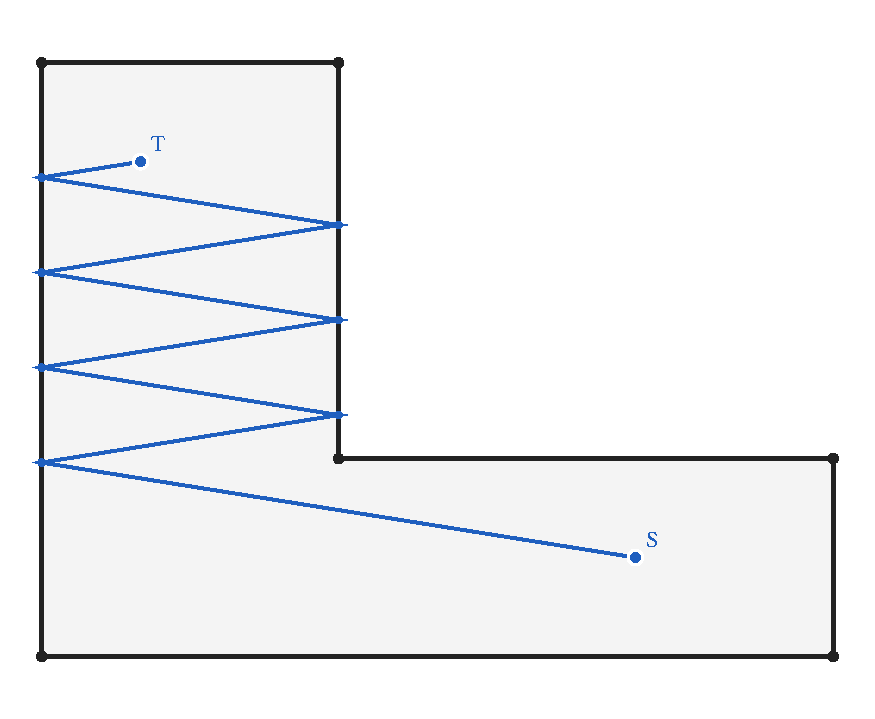
\includegraphics[width=0.70\linewidth,height=0.30\textheight,keepaspectratio]{figures/fig-L.pdf}\caption{An L-room path with controlled reflection orientation (Theorem 2.1).}\end{figure}
\begin{figure}[htbp]\centering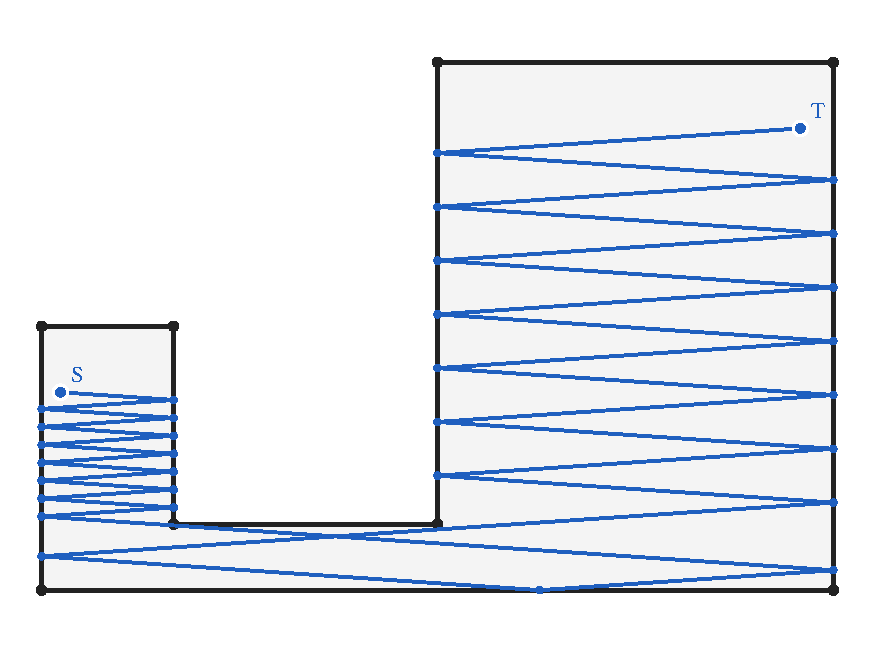
\includegraphics[width=0.70\linewidth,height=0.30\textheight,keepaspectratio]{figures/fig-U.pdf}\caption{The opposite-arm U construction, with one smooth floor reflection (Theorem 3.1).}\end{figure}
\begin{figure}[htbp]\centering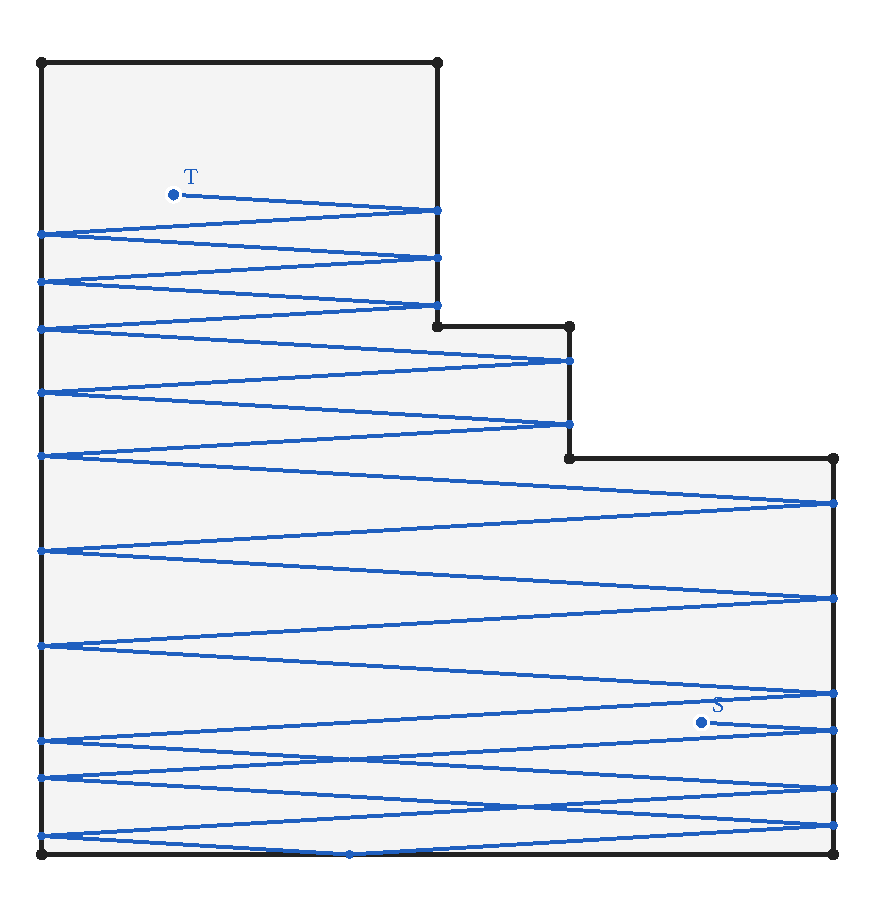
\includegraphics[width=0.70\linewidth,height=0.30\textheight,keepaspectratio]{figures/fig-staircase-floor.pdf}\caption{The staircase floor chart (Theorem 6.5).}\end{figure}
\begin{figure}[htbp]\centering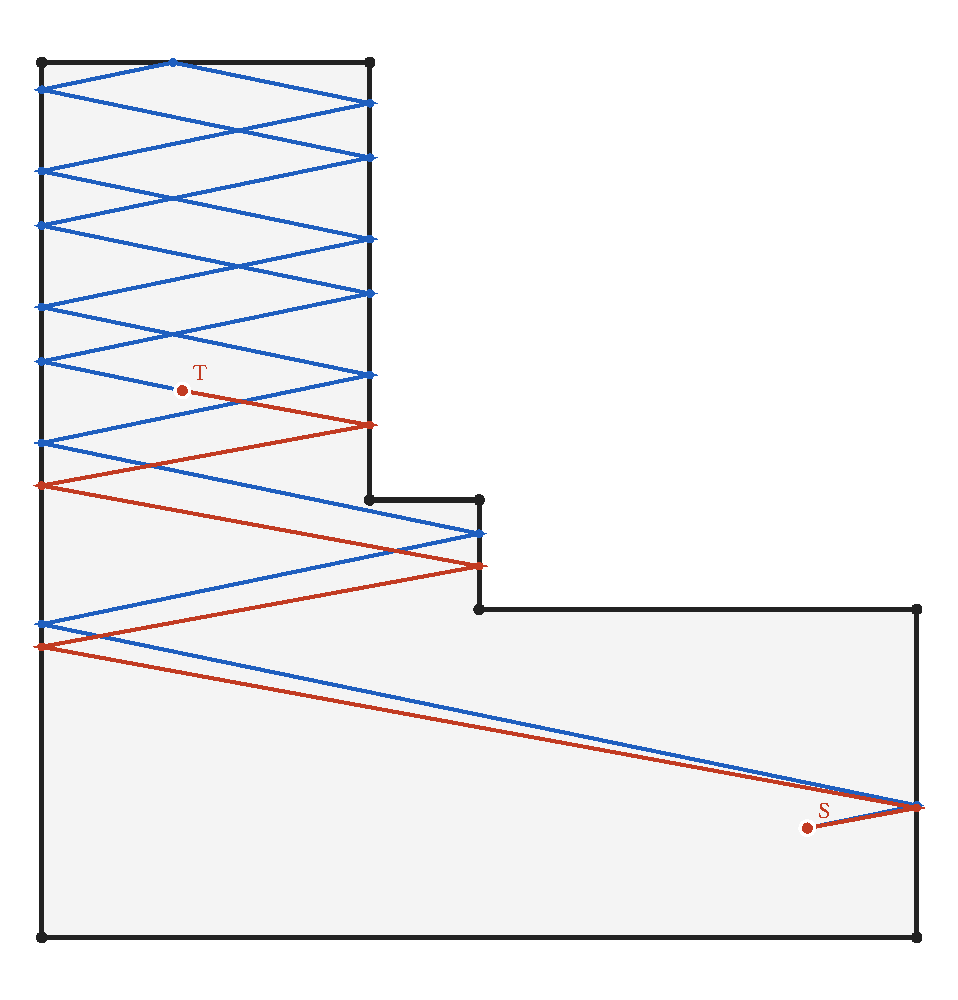
\includegraphics[width=0.70\linewidth,height=0.30\textheight,keepaspectratio]{figures/fig-staircase-roof.pdf}\caption{The roof chart (Theorem 6.8). The blue path has a smooth roof reflection; the red path reaches the target before its candidate roof-corner contact and stops there.}\end{figure}
\end{document}
